\documentclass[12pt,a4paper]{extarticle}
\usepackage[margin=1in]{geometry}
\usepackage[slantfont,boldfont]{xeCJK}
\usepackage{graphicx}
\usepackage{caption}
\usepackage{float}
\usepackage{pgfplots}
\usepackage{subcaption}

\graphicspath{{./images/}}
\pgfplotsset{compat=1.12}
\setCJKmainfont{cwTeXKai}

\title{Machine Learning 2017 Spring\\Homework 4 Report}
\author{學號:\texttt{B03902048}\\系級:資工三\\姓名:林義聖}
\date{}

\begin{document}
\maketitle

\section{Eigenfaces with PCA}

\begin{figure}[ht]
  \centering
  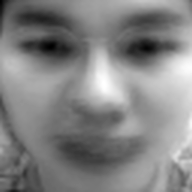
\includegraphics[width=0.4\linewidth]{average-face.png}
  \caption{The average face}
  \label{fig:average-face}
\end{figure}

\begin{figure}[ht]
  \centering
  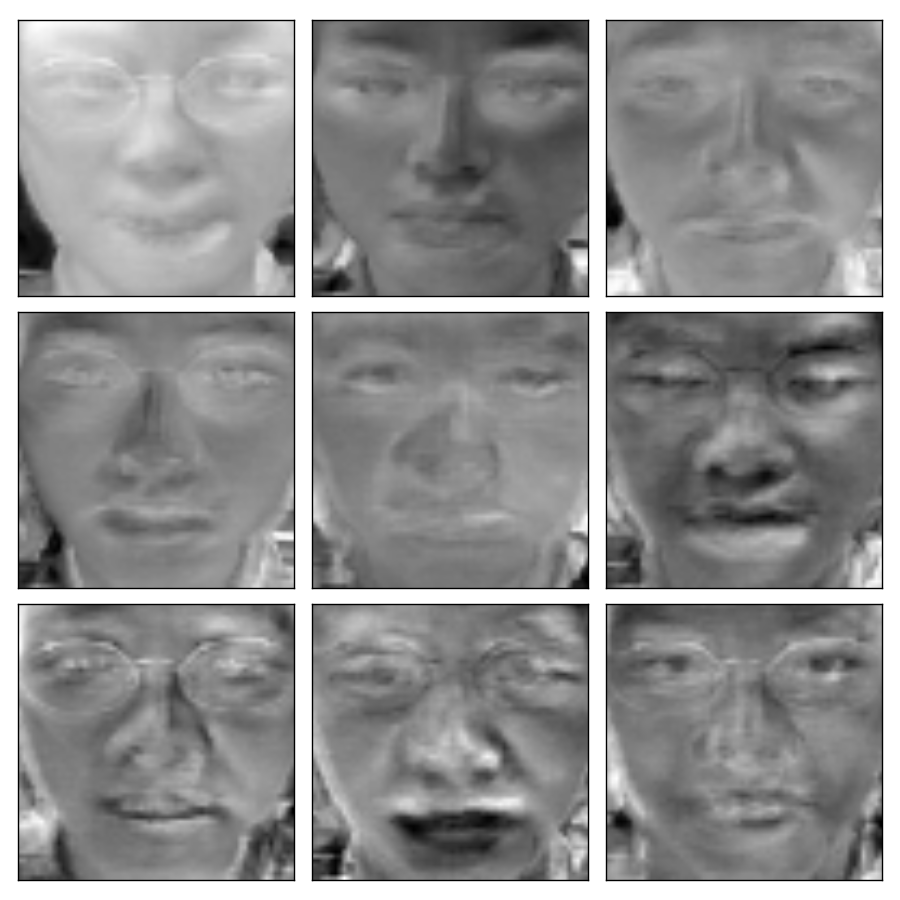
\includegraphics[width=0.6\linewidth]{eigen-faces-top-9.png}
  \caption{The top 9 eigenfaces}
  \label{fig:top-9-eigenfaces}
\end{figure}

\begin{figure}[ht]
  \centering
  \begin{tikzpicture}
    \begin{axis}[
      ytick={0, 0.01, 0.02, 0.03, 0.04, 0.05, 0.06, 0.07, 0.08, 0.09, 0.1},
      xlabel = \# of eigenfaces,
      ymajorgrids]
    \addplot[color=blue] table [x=nb, y=rate, col sep=comma] {reconstruct-error.csv};
    \end{axis}
  \end{tikzpicture}
  \caption{Reconstruction error (RMSE)}
  \label{fig:eigenfaces-error-rate}
\end{figure}

\begin{figure}[ht]
  \begin{subfigure}[t]{0.5\textwidth}
    \centering
    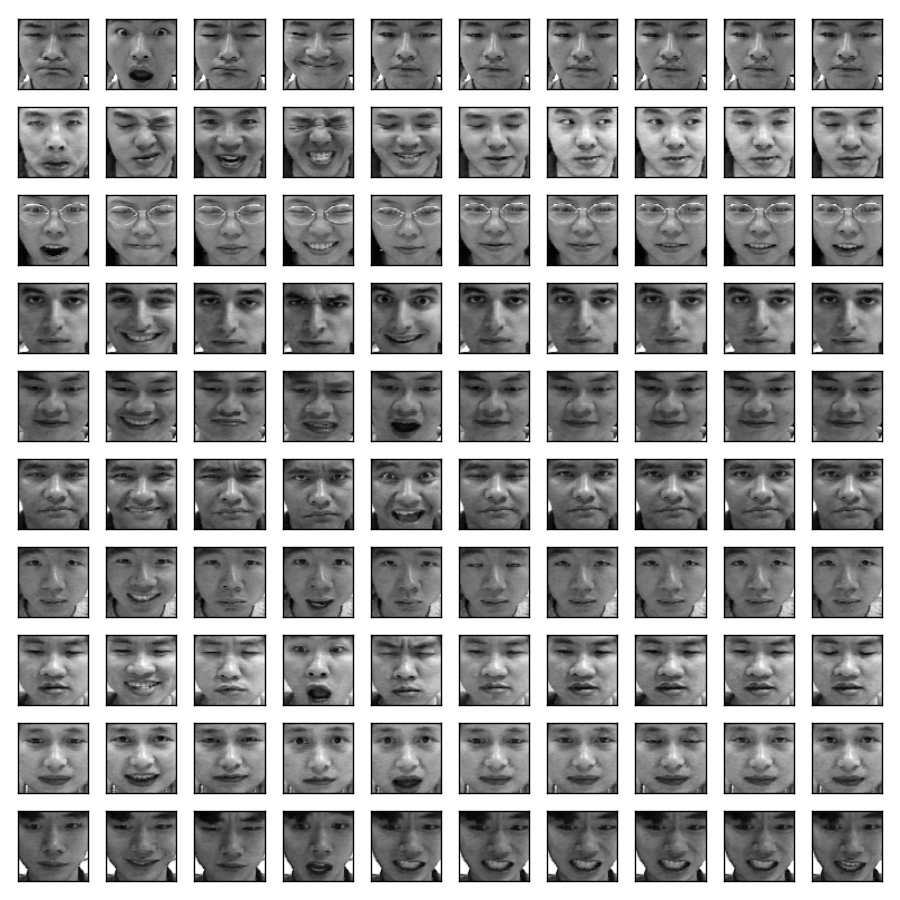
\includegraphics[width=\linewidth]{origin-faces-first-100.png}
    \caption{Original faces}
    \label{fig:original-faces}
  \end{subfigure}
  \begin{subfigure}[t]{0.5\textwidth}
    \centering
    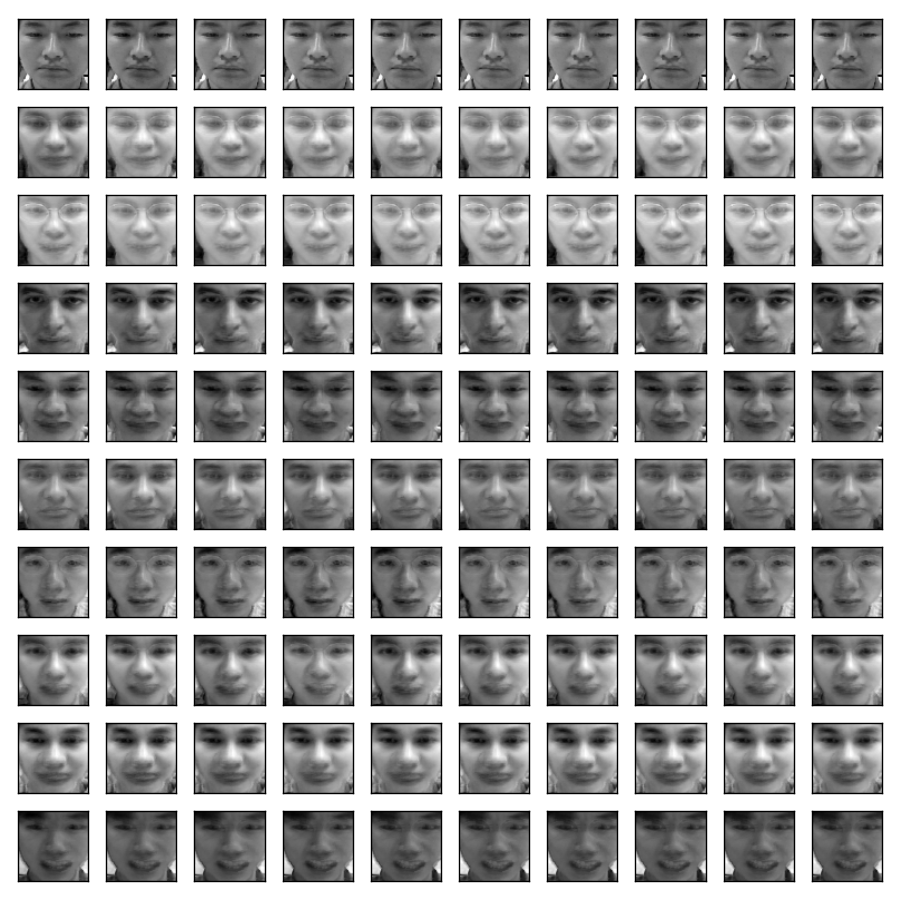
\includegraphics[width=\linewidth]{reconstruct-with-5-eigenfaces.png}
    \caption{Recovered faces}
    \label{fig:recovered-faces}
  \end{subfigure}
  \caption{100 faces reconstructed with top 5 eigenfaces}
  \label{fig:reconstruct-with-eigenfaces}
\end{figure}

  % \begin{table}[ht]
  %   \centering
  %   \caption{Probability distribution}
  %   \label{tab:prob-distribution}
  %   \begin{tabular}{|c|c|c|c|c|c|c|c|}\hline
  %   \# & Angry & Disgust & Fear & Happy & Sad & Surprice & Neutral \\\hline
  %   Figure \ref{fig:train-image-2} & 0.06 & 0 & 0.07 & 0 & 0.87 & 0 & 0 \\\hline
  %   Figure \ref{fig:train-image-6} & 0 & 0 & 0.48 & 0 & 0.44 & 0 & 0.08 \\\hline
  %   \end{tabular}
  % \end{table}

\end{document}
